\newpage
\section*{Математическая постановка задачи}

Предположим, у нас есть ненаправленная антенна, представляемая точечным источником (расстояние до поверхности значительно больше размеров антенны) с излучающей мощностью $P_0$. Тогда вся энергия распределяется равномерно по всей поверхности некоторой сферы радиуса $R$, площадь поверхности которой равна $ 4 \pi R^2 $. Таким образом, источник электромагнитного излучения создает плотность потока мощности
\begin{gather}
   J = \frac{P_0}{4 \pi R^2}
\end{gather}
Следовательно, каждая точка поверхности $ M(x, y, z) $, которая располагается в зоне прямой видимости, получает от источника излучения в секунду энергию мощности на единицу площади равную
\begin{gather}
  dP_{in} =   \left\langle  {\vec{J}(x,y,z) \cdot  \vec{d\sigma} } \right\rangle = J(x,y,z) \cdot d\sigma \cdot cos \phi ,
\end{gather}
где $d\sigma$ -- окрестность точки $ M(x, y, z) $, а $\phi$ -- угол между вектором $ \vec{J}(M) $ и нормалью к поверхности $d\sigma$, направленной в противоположную сторону от источника излучения.  

Значит, учитывая $(4)$, первично-освещенная поверхность получает в секунду энергию мощности, равную 
\begin{gather}
  P_{in} =   \int \limits_S \left\langle  {\vec{J}(x,y,z) \cdot  \vec{d\sigma} } \right\rangle,
\end{gather}
где $ S $ -- первично-освещенная поверхность.

Часть энергии попадаемые в точки первично-освещенных поверхностей поглощается, часть отражается. Точки, отражающие электромагнитные волны ведут себя как вторичные источники электромагнитного излучения, а значит вышепроделанные умозаключения к ним тоже применимы. 

После многократного отражения и переотражения получаем, что для каждой точки $ M(x,y,z) $ справедливо
\begin{gather}
  J_{out}(x,y,z,\vec \omega) = \int \limits_\Omega J_{in}(x,y,z,\vec \theta) \cdot f(x,y,z,\vec \omega,\vec \theta) \cdot \left\langle  {-\vec \theta \cdot \vec n} \right\rangle \cdot d\theta,
\end{gather}

где $ J_{out} $ -- поток из точки $(x,y,z)$ в направлении вектора $ \vec \omega $, а $ J_{in} $ -- поток входящего в точку $(x,y,z)$ излучения из направления вектора $ \vec \theta $. В данном уравнении интеграл взят по $ \Omega $ -- совокупности входящих направлений в точку $M(x,y,z)$, $\theta$ -- телесный угол, порожденный вектором $\vec \theta$. Способ отражения от поверхности, а также соотношение отраженной энергии и поглощенной задано в общем случае двулучевой функцией отражения $ f(x,y,z,\vec \omega,\vec \theta) $. 

\begin{center}
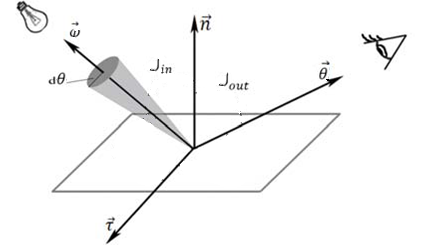
\includegraphics[width=0.499\linewidth]{rendering-equation.png}
\end{center}

Уравнение $(6)$ является частным случаем более общего уравнения, называемого уравнением рендеринга  \cite{rendering-equ}. Существует несколько подходов к его решению. Рассмотрим их.
